\documentclass[11pt, a4paper]{article}

% Mandatory Packages
\usepackage{amsmath}
\usepackage{amssymb}
\usepackage{amsthm}
\usepackage{geometry}
\usepackage{tikz}
\usetikzlibrary{arrows.meta, positioning, shapes.geometric, calc}
\usepackage{mathrsfs}
\usepackage{mathtools}
\usepackage{hyperref}
\usepackage{enumitem}
\usepackage{xcolor}

% Page Geometry
\geometry{
    top=1in,
    bottom=1in,
    left=1in,
    right=1in
}

% Theorem Environments
\newtheorem{theorem}{Theorem}[section]
\newtheorem{lemma}[theorem]{Lemma}
\newtheorem{proposition}[theorem]{Proposition}
\newtheorem{corollary}[theorem]{Corollary}
\theoremstyle{definition}
\newtheorem{definition}{Definition}[section]
\newtheorem{axiom}{Axiom}[section]
\newtheorem{example}{Example}[section]
\theoremstyle{remark}
\newtheorem{remark}{Remark}[section]

% Custom Commands
\newcommand{\R}{\mathbb{R}}
\newcommand{\Z}{\mathbb{Z}}
\newcommand{\N}{\mathbb{N}}
\newcommand{\Q}{\mathbb{Q}}
\newcommand{\E}{\mathbb{E}}
\newcommand{\Prob}{\mathbb{P}}
\newcommand{\F}{\mathcal{F}}
\newcommand{\ind}{\mathbf{1}}

% Document Metadata
\title{\textbf{Homework 5: A Review of Three Proof Techniques}}
\author{Tashfeen Omran}
\date{September 2026}

\begin{document}

\maketitle
\tableofcontents
\newpage

% ==========================================
% PART 1: Introduction, Context, and Prerequisites
% ==========================================
\section{Part 1: Comprehensive Introduction, Context, and Prerequisites}

\subsection{Core Concepts \& Axioms}
In the formal study of abstract mathematics, establishing the absolute truth of a proposition requires rigorous logical deduction from a set of accepted axioms. Section 5.3 synthesizes the three foundational pillars of mathematical verification for conditional statements of the form $P \implies Q$ (read as ``If $P$, then $Q$''):
\begin{enumerate}
    \item \textbf{Direct Proof:} We assume the hypothesis $P$ is true. Through a sequence of logically valid deductions, algebraic manipulations, and applications of previously proven theorems, we demonstrate that the conclusion $Q$ must necessarily be true.
    \item \textbf{Proof by Contrapositive:} This technique relies on the logical equivalence between a conditional statement and its contrapositive: $(P \implies Q) \equiv (\sim Q \implies \sim P)$. We assume the negation of the conclusion ($\sim Q$) and logically deduce the negation of the hypothesis ($\sim P$).
    \item \textbf{Proof by Contradiction (Reductio ad Absurdum):} We assume that the entire conditional statement is false. The only way $P \implies Q$ can be false is if the hypothesis $P$ is true and the conclusion $Q$ is false. Thus, we assume $P \land \sim Q$. We then deduce a logical impossibility or contradiction (denoted $C$), such as $0 = 1$ or $R \land \sim R$. Since our assumption led to an absurdity, the original statement must be true.
\end{enumerate}

\subsection{Intuition and Set-Theoretic Foundations}
From a set-theoretic perspective, consider a domain $S$ and subsets $A = \{x \in S \mid P(x) \text{ is true}\}$ and $B = \{x \in S \mid Q(x) \text{ is true}\}$. The statement $\forall x \in S, P(x) \implies Q(x)$ is equivalent to asserting that $A \subseteq B$. 
\begin{itemize}
    \item A \textbf{Direct Proof} takes an arbitrary element $x \in A$ and shows it must also reside in $B$.
    \item A \textbf{Proof by Contrapositive} takes an arbitrary element $x \notin B$ (i.e., $x \in B^c$) and shows it cannot reside in $A$ (i.e., $x \in A^c$). This establishes $B^c \subseteq A^c$, which is set-theoretically equivalent to $A \subseteq B$.
    \item A \textbf{Proof by Contradiction} assumes there exists an element $x$ such that $x \in A$ and $x \notin B$ (i.e., $A \cap B^c \neq \emptyset$). We then show that the existence of such an element violates the fundamental axioms of the space $S$, proving that $A \cap B^c = \emptyset$, which implies $A \subseteq B$.
\end{itemize}

\subsection{Historical Context and Motivation}
The formalization of these proof techniques dates back to ancient Greek mathematics, most notably Euclid's \textit{Elements} and Aristotle's formulation of the Law of the Excluded Middle ($P \lor \sim P$) and the Principle of Non-Contradiction ($\sim(P \land \sim P)$). Proof by contradiction was famously used by the Pythagoreans to prove the irrationality of $\sqrt{2}$, a discovery that caused a foundational crisis in their worldview, which assumed all quantities could be expressed as ratios of integers. In modern times, these techniques form the bedrock of formal verification in computer science, automated theorem proving, and the rigorous foundations of probability theory (e.g., Kolmogorov's axioms).

\subsection{Key Theorems and Logical Equivalences}
\begin{theorem}[Logical Equivalences for Proofs]
Let $P$ and $Q$ be logical propositions.
\begin{align}
    (P \implies Q) &\equiv (\sim Q \implies \sim P) \quad \text{(Contrapositive)} \\
    \sim(P \implies Q) &\equiv (P \land \sim Q) \quad \text{(Negation of Implication)} \\
    (P \implies Q) &\equiv \sim(P \land \sim Q) \quad \text{(Basis for Contradiction)}
\end{align}
\end{theorem}

\subsection{Prerequisites}
To master this section, the reader must possess:
\begin{itemize}
    \item \textbf{Propositional Logic:} Fluency in De Morgan's Laws and negating quantified statements (e.g., $\sim(\forall x, P(x)) \equiv \exists x, \sim P(x)$).
    \item \textbf{Number Theory Basics:} Formal definitions of even integers ($n = 2k, k \in \Z$) and odd integers ($n = 2k+1, k \in \Z$).
    \item \textbf{Real Analysis Basics:} Properties of inequalities, particularly behavior under multiplication by negative numbers, and the definition of positive real numbers ($\R^+$).
\end{itemize}

% ==========================================
% PART 2: Detailed Homework Solutions
% ==========================================
\section{Part 2: Detailed Homework Solutions}

\subsection{Exercise 5.36}
\textbf{Problem:} Prove that if $n$ is an odd integer, then $7n - 5$ is even by (a) a direct proof, (b) a proof by contrapositive, and (c) a proof by contradiction.

\begin{proof}[\textbf{Solution (a): Direct Proof}]
Let $n$ be an arbitrary odd integer. By definition of an odd integer, there exists some integer $k \in \Z$ such that $n = 2k + 1$. We substitute this expression into the target polynomial:
\begin{align*}
    7n - 5 &= 7(2k + 1) - 5 \\
           &= 14k + 7 - 5 \\
           &= 14k + 2 \\
           &= 2(7k + 1)
\end{align*}
Since $k \in \Z$, the set of integers is closed under multiplication and addition, meaning $(7k + 1) \in \Z$. Let $m = 7k + 1$. Then $7n - 5 = 2m$ for $m \in \Z$. By definition, $7n - 5$ is an even integer.
\end{proof}

\begin{proof}[\textbf{Solution (b): Proof by Contrapositive}]
We aim to prove the contrapositive: If $7n - 5$ is an odd integer, then $n$ is an even integer. 
Assume $7n - 5$ is an odd integer. By definition, there exists an integer $k \in \Z$ such that:
\[ 7n - 5 = 2k + 1 \]
Adding $5$ to both sides yields:
\[ 7n = 2k + 6 \]
To isolate $n$ algebraically while maintaining integer coefficients, we can subtract $6n$ from both sides:
\begin{align*}
    7n - 6n &= 2k + 6 - 6n \\
    n &= 2(k + 3 - 3n)
\end{align*}
Since $k, n \in \Z$, the expression $(k + 3 - 3n)$ is an integer. Let $m = k + 3 - 3n$. Thus, $n = 2m$ for $m \in \Z$, which means $n$ is an even integer. This proves the contrapositive, and hence the original statement is true.
\end{proof}

\begin{proof}[\textbf{Solution (c): Proof by Contradiction}]
Assume, to the contrary, that the statement is false. That is, assume there exists an integer $n$ such that $n$ is odd AND $7n - 5$ is odd.
Since $n$ is odd, there exists $k \in \Z$ such that $n = 2k + 1$. Substituting this into $7n - 5$:
\begin{align*}
    7n - 5 &= 7(2k + 1) - 5 \\
           &= 14k + 2 \\
           &= 2(7k + 1)
\end{align*}
This shows that $7n - 5$ is a multiple of 2, meaning it is an even integer. However, our initial assumption stated that $7n - 5$ is an odd integer. An integer cannot be both even and odd simultaneously (a contradiction). Therefore, our assumption must be false, and the original statement is true.
\end{proof}

\subsection{Exercise 5.37}
\textbf{Problem:} Let $x$ be a positive real number. Prove that if $x - \frac{2}{x} > 1$, then $x > 2$ by (a) a direct proof, (b) a proof by contrapositive, and (c) a proof by contradiction.

\begin{proof}[\textbf{Solution (a): Direct Proof}]
Let $x \in \R^+$ (so $x > 0$). Assume $x - \frac{2}{x} > 1$. 
Since $x > 0$, we can multiply both sides of the inequality by $x$ without changing the direction of the inequality:
\begin{align*}
    x\left(x - \frac{2}{x}\right) &> x(1) \\
    x^2 - 2 &> x \\
    x^2 - x - 2 &> 0
\end{align*}
Factoring the quadratic expression yields:
\[ (x - 2)(x + 1) > 0 \]
Since $x > 0$, it follows that $x + 1 > 1 > 0$. Because the product $(x - 2)(x + 1)$ is strictly positive and the factor $(x + 1)$ is strictly positive, we can divide both sides by $(x + 1)$ without flipping the inequality:
\[ x - 2 > 0 \implies x > 2 \]
This completes the direct proof.
\end{proof}

\begin{proof}[\textbf{Solution (b): Proof by Contrapositive}]
We aim to prove the contrapositive: Let $x \in \R^+$. If $x \leq 2$, then $x - \frac{2}{x} \leq 1$.
Assume $x \leq 2$. Since $x$ is a positive real number, we have $0 < x \leq 2$. 
Because $x \leq 2$ and $x > 0$, taking the reciprocal reverses the inequality:
\[ \frac{1}{x} \geq \frac{1}{2} \]
Multiplying by $-2$ reverses the inequality again:
\[ -\frac{2}{x} \leq -1 \]
We also know that $x \leq 2$. Adding these two inequalities ($x \leq 2$ and $-\frac{2}{x} \leq -1$) yields:
\[ x - \frac{2}{x} \leq 2 - 1 \]
\[ x - \frac{2}{x} \leq 1 \]
This proves the contrapositive.
\end{proof}

\begin{proof}[\textbf{Solution (c): Proof by Contradiction}]
Assume, to the contrary, that there exists a positive real number $x \in \R^+$ such that $x - \frac{2}{x} > 1$ AND $x \leq 2$.
From the assumption $x \leq 2$ and knowing $x > 0$, we can deduce bounds on $-\frac{2}{x}$. 
Since $x \leq 2$, we have $\frac{1}{x} \geq \frac{1}{2}$, which implies $-\frac{2}{x} \leq -1$.
Adding $x$ to both sides of this inequality gives:
\[ x - \frac{2}{x} \leq x - 1 \]
Since we assumed $x \leq 2$, we can substitute this upper bound for $x$:
\[ x - \frac{2}{x} \leq 2 - 1 = 1 \]
Thus, we have deduced that $x - \frac{2}{x} \leq 1$. However, our initial assumption explicitly stated that $x - \frac{2}{x} > 1$. This is a contradiction ($1 < x - \frac{2}{x} \leq 1$). Therefore, the original statement must be true.
\end{proof}

\subsection{Exercise 5.38}
\textbf{Problem:} Let $a, b \in \R$. Prove that if $ab \neq 0$, then $a \neq 0$ by using more than one proof technique.

\begin{proof}[\textbf{Method 1: Proof by Contrapositive}]
The contrapositive of the statement is: If $a = 0$, then $ab = 0$.
Assume $a = 0$. By the zero property of multiplication for real numbers, substituting $a = 0$ into the expression $ab$ yields:
\[ ab = (0)b = 0 \]
Thus, $ab = 0$. The contrapositive is true, hence the original statement is true.
\end{proof}

\begin{proof}[\textbf{Method 2: Proof by Contradiction}]
Assume, to the contrary, that there exist real numbers $a, b \in \R$ such that $ab \neq 0$ AND $a = 0$.
Substituting $a = 0$ into the product $ab$, we get:
\[ ab = (0)b = 0 \]
This implies $ab = 0$. However, our assumption states that $ab \neq 0$. This is a direct contradiction ($0 \neq 0$). Therefore, the assumption is false, and the original statement holds.
\end{proof}

\subsection{Exercise 5.39}
\textbf{Problem:} Let $x, y \in \R^+$. Prove that if $x \leq y$, then $x^2 \leq y^2$ by (a) a direct proof, (b) a proof by contrapositive, and (c) a proof by contradiction.

\begin{proof}[\textbf{Solution (a): Direct Proof}]
Let $x, y \in \R^+$. Assume $x \leq y$. 
Since $x > 0$, multiplying both sides of $x \leq y$ by $x$ preserves the inequality:
\[ x^2 \leq xy \]
Similarly, since $y > 0$, multiplying both sides of $x \leq y$ by $y$ preserves the inequality:
\[ xy \leq y^2 \]
By the transitive property of inequalities, since $x^2 \leq xy$ and $xy \leq y^2$, it follows that:
\[ x^2 \leq y^2 \]
\end{proof}

\begin{proof}[\textbf{Solution (b): Proof by Contrapositive}]
We aim to prove the contrapositive: Let $x, y \in \R^+$. If $x^2 > y^2$, then $x > y$.
Assume $x^2 > y^2$. Subtracting $y^2$ from both sides yields:
\[ x^2 - y^2 > 0 \]
Factoring the difference of squares gives:
\[ (x - y)(x + y) > 0 \]
Since $x, y \in \R^+$, we know $x > 0$ and $y > 0$, which implies their sum is strictly positive: $x + y > 0$. 
Dividing both sides of the inequality by the positive quantity $(x + y)$ preserves the inequality direction:
\[ x - y > 0 \implies x > y \]
This proves the contrapositive.
\end{proof}

\begin{proof}[\textbf{Solution (c): Proof by Contradiction}]
Assume, to the contrary, that there exist $x, y \in \R^+$ such that $x \leq y$ AND $x^2 > y^2$.
From the assumption $x \leq y$, and knowing $x, y > 0$, we can multiply the inequality by $x$ and $y$ respectively to obtain:
\[ x^2 \leq xy \quad \text{and} \quad xy \leq y^2 \]
By transitivity, this implies:
\[ x^2 \leq y^2 \]
However, our initial assumption explicitly stated that $x^2 > y^2$. This is a contradiction. Therefore, the original statement must be true.
\end{proof}

% ==========================================
% PART 3: In-Depth Analysis of Problems
% ==========================================
\section{Part 3: In-Depth Analysis of Problems and Techniques}

\subsection{A) Problem Types and Logical Strategies}
The problems in Section 5.3 fall into two primary categories:
\begin{enumerate}
    \item \textbf{Number-Theoretic Parity Proofs (e.g., 5.36):} These problems deal with the discrete domain of integers ($\Z$). The overarching strategy is algebraic substitution using the definitions of even ($2k$) and odd ($2k+1$). The goal is to factor out a $2$ to demonstrate parity.
    \item \textbf{Real Analysis Inequality Proofs (e.g., 5.37, 5.39):} These problems deal with the continuous domain of positive real numbers ($\R^+$). The strategy relies heavily on the order axioms of $\R$. A critical component is recognizing that multiplying or dividing by a variable requires strict knowledge of its sign to determine if the inequality direction is preserved or reversed.
\end{enumerate}

\subsection{B) Key Analytical and Logical Manipulations}
\begin{itemize}
    \item \textbf{The ``Isolate the Variable'' Trick in Contrapositive (5.36b):} When proving $7n - 5 = 2k + 1 \implies n = 2m$, standard division yields $n = \frac{2k+6}{7}$, which introduces fractions and breaks the integer closure property. The trick used was subtracting $6n$ from both sides: $7n - 6n = 2k + 6 - 6n \implies n = 2(k + 3 - 3n)$. This elegantly maintains integer coefficients.
    \item \textbf{Exploiting Domain Constraints (5.37a, 5.39b):} In 5.37a, we reached $(x-2)(x+1) > 0$. In general algebra, this requires testing intervals. However, the domain constraint $x \in \R^+$ guarantees $x+1 > 0$, allowing us to divide it out immediately. This highlights the importance of stating domain assumptions explicitly.
    \item \textbf{Transitivity of Inequalities (5.39a):} A common technique to prove $A \leq C$ is to construct an intermediate term $B$ such that $A \leq B$ and $B \leq C$. In 5.39a, $xy$ served as the perfect intermediate term.
\end{itemize}

% ==========================================
% PART 4: Cheatsheet, Visuals, and Tips
% ==========================================
\section{Part 4: ``Cheatsheet'', Visuals, and Tips for Success}

\subsection{Theorems \& Equivalences Summary}
\begin{center}
\renewcommand{\arraystretch}{1.5}
\begin{tabular}{|l|l|l|}
\hline
\textbf{Technique} & \textbf{Assume} & \textbf{Goal (Deduce)} \\
\hline
Direct Proof & $P$ is true & $Q$ is true \\
Contrapositive & $\sim Q$ is true & $\sim P$ is true \\
Contradiction & $P$ is true AND $\sim Q$ is true & A contradiction $C$ (e.g., $R \land \sim R$) \\
\hline
\end{tabular}
\end{center}

\subsection{Visualizing Proof Techniques}
The following TikZ diagram illustrates the logical pathways of the three proof techniques when attempting to prove $P \implies Q$.

\begin{center}
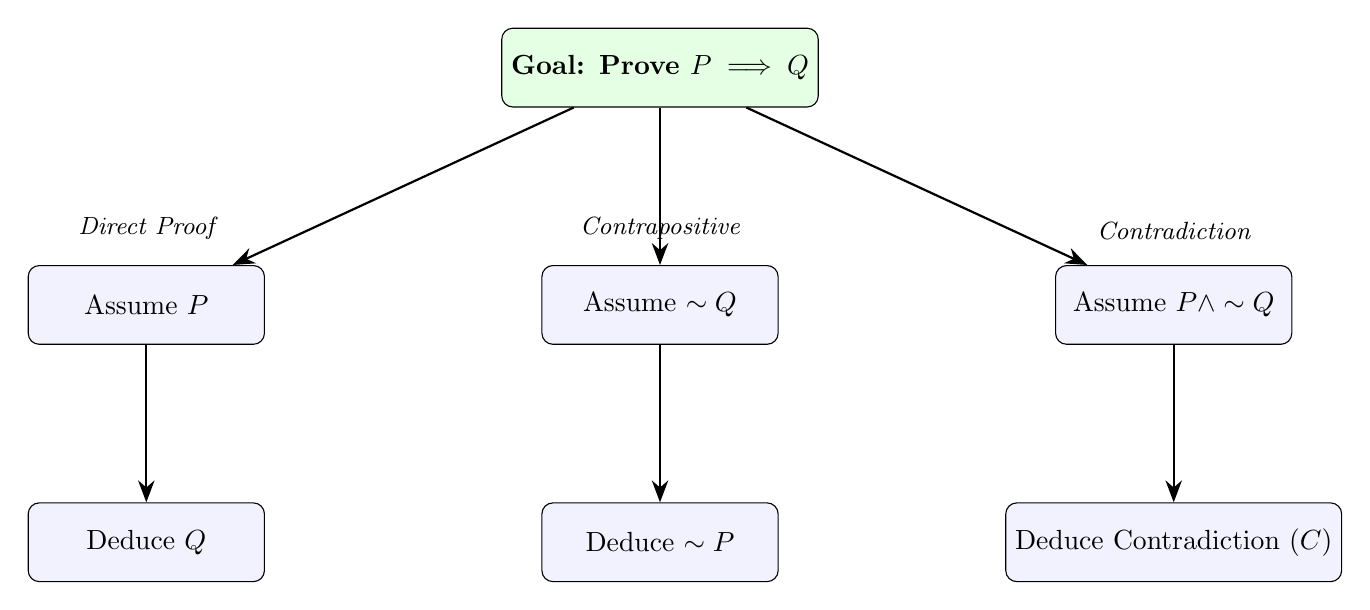
\begin{tikzpicture}[
    node distance=2cm and 3cm,
    box/.style={draw, rectangle, rounded corners, minimum width=3cm, minimum height=1cm, align=center, fill=blue!5},
    arrow/.style={-{Stealth[scale=1.2]}, thick}
]

% Nodes
\node[box, fill=green!10, font=\bfseries] (start) {Goal: Prove $P \implies Q$};

\node[box, below left=of start] (direct_ass) {Assume $P$};
\node[box, below=of direct_ass] (direct_goal) {Deduce $Q$};

\node[box, below=of start] (contra_ass) {Assume $\sim Q$};
\node[box, below=of contra_ass] (contra_goal) {Deduce $\sim P$};

\node[box, below right=of start] (contra_dict_ass) {Assume $P \land \sim Q$};
\node[box, below=of contra_dict_ass] (contra_dict_goal) {Deduce Contradiction ($C$)};

% Labels
\node[above=0.2cm of direct_ass, font=\itshape\small] {Direct Proof};
\node[above=0.2cm of contra_ass, font=\itshape\small] {Contrapositive};
\node[above=0.2cm of contra_dict_ass, font=\itshape\small] {Contradiction};

% Arrows
\draw[arrow] (start) -- (direct_ass);
\draw[arrow] (start) -- (contra_ass);
\draw[arrow] (start) -- (contra_dict_ass);

\draw[arrow] (direct_ass) -- (direct_goal);
\draw[arrow] (contra_ass) -- (contra_goal);
\draw[arrow] (contra_dict_ass) -- (contra_dict_goal);

\end{tikzpicture}
\end{center}

\subsection{Heuristics \& ``Cheats''}
\begin{itemize}
    \item \textbf{When to use Contrapositive:} If the conclusion $Q$ contains negative phrasing (e.g., ``$x \neq 0$'', ``$n$ is not divisible by 3''), negating it for a contrapositive proof turns it into a positive, workable assumption (e.g., ``$x = 0$'', ``$n = 3k$'').
    \item \textbf{When to use Contradiction:} Highly effective for proving non-existence, irrationality, or uniqueness. If a problem says ``Prove there is no $x$ such that...'', immediately assume such an $x$ exists and find the contradiction.
\end{itemize}

\subsection{Pitfalls \& Fallacies}
\begin{itemize}
    \item \textbf{Affirming the Consequent:} Assuming $Q$ to prove $P$. This proves $Q \implies P$, which is the converse, not the original statement.
    \item \textbf{Denying the Antecedent:} Assuming $\sim P$ to prove $\sim Q$. This proves the inverse, which is logically equivalent to the converse, not the original statement.
    \item \textbf{Circular Reasoning (Begging the Question):} Using the conclusion $Q$ as an implicit assumption during the algebraic manipulation of a direct proof.
\end{itemize}

% ==========================================
% PART 5: Conceptual Synthesis
% ==========================================
\section{Part 5: Conceptual Synthesis and The ``Big Picture''}

\subsection{A) Thematic Connections}
The central theme of this section is \textbf{logical isomorphism}. Just as two algebraic structures can be isomorphic (structurally identical despite different elements), logical statements can be isomorphic via truth tables. The equivalence $(P \implies Q) \equiv (\sim Q \implies \sim P)$ allows mathematicians to map a difficult problem into an isomorphic space where the algebra is easier to manipulate, solve it there, and map the truth back to the original problem.

\subsection{B) Forward and Backward Links}
\begin{itemize}
    \item \textbf{Backward Links:} This topic relies heavily on the foundational set theory and propositional logic established in Chapters 1-3. The manipulation of inequalities relies on the field axioms of the real numbers.
    \item \textbf{Forward Links:} Mastering these three techniques is the absolute prerequisite for advanced mathematics. In Real Analysis, proving that a sequence converges often uses direct proofs ($\epsilon-\delta$ definitions), while proving a sequence diverges often uses contradiction. In Measure Theory, proving that a set is measurable often relies on contrapositive arguments regarding its complement.
\end{itemize}

% ==========================================
% PART 6: Abstract Real-World Modeling
% ==========================================
\section{Part 6: Abstract Real-World Modeling (AI, ML, \& Quant Finance)}

\subsection{A) Concrete Scenarios}
\begin{enumerate}
    \item \textbf{Quantitative Finance (Arbitrage Pricing Theory):} The Fundamental Theorem of Asset Pricing states that a market is arbitrage-free if and only if there exists a risk-neutral probability measure. Proofs in this domain almost exclusively use \textbf{Proof by Contradiction}. A quant will assume an arbitrage opportunity exists (a portfolio with zero initial cost, zero probability of loss, and positive probability of profit) and deduce that this leads to infinite wealth generation, contradicting market equilibrium constraints.
    \item \textbf{Machine Learning (Statistical Learning Theory):} When proving bounds on the generalization error of a classifier (e.g., PAC learning), researchers often use \textbf{Proof by Contrapositive}. Statement: ``If the sample size $N$ is sufficiently large, the empirical risk converges to the true risk.'' Contrapositive: ``If the empirical risk diverges from the true risk, the sample size $N$ must be bounded/small.''
\end{enumerate}

\subsection{B) Model Problem Setup: Arbitrage in a Binomial Model}
Let us formalize a scenario in Quantitative Finance using Proof by Contradiction.

\textbf{Definitions \& State Space:}
Consider a one-period financial market with two assets: a risk-free bank account $B$ and a risky stock $S$. 
Let the current time be $t=0$ and the future time be $t=1$.
The state space at $t=1$ is $\Omega = \{\omega_{up}, \omega_{down}\}$.
\begin{itemize}
    \item $B_0 = 1$, and $B_1 = 1 + r$, where $r > 0$ is the risk-free rate.
    \item $S_0 > 0$ is the initial stock price.
    \item $S_1(\omega_{up}) = u S_0$ and $S_1(\omega_{down}) = d S_0$, where $0 < d < u$.
\end{itemize}

\textbf{Theorem:} To prevent arbitrage, it must be strictly true that $d < 1+r < u$.

\begin{proof}[Proof by Contradiction]
Assume, to the contrary, that the market is arbitrage-free, but the condition $d < 1+r < u$ is false. 
Without loss of generality, assume $1+r \leq d < u$. (The case $d < u \leq 1+r$ is symmetric).
We construct a portfolio $\Pi$ at $t=0$ by borrowing $S_0$ dollars from the bank (shorting the bond) and buying 1 share of the stock.
The initial wealth is $X_0 = S_0 - S_0 = 0$.
At $t=1$, the value of the portfolio is $X_1(\omega) = S_1(\omega) - S_0(1+r)$.
Evaluate $X_1$ in both states:
\begin{align*}
    X_1(\omega_{up}) &= u S_0 - S_0(1+r) = S_0(u - (1+r)) \\
    X_1(\omega_{down}) &= d S_0 - S_0(1+r) = S_0(d - (1+r))
\end{align*}
Since we assumed $1+r \leq d < u$, it follows that $u - (1+r) > 0$ and $d - (1+r) \geq 0$.
Because $S_0 > 0$, we have $X_1(\omega_{up}) > 0$ and $X_1(\omega_{down}) \geq 0$.
Thus, $\Prob(X_1 \geq 0) = 1$ and $\Prob(X_1 > 0) > 0$.
This portfolio requires zero initial investment ($X_0 = 0$) but guarantees a non-negative payoff with a strictly positive probability of profit. By definition, this is an arbitrage opportunity.
However, we assumed the market is arbitrage-free. This is a contradiction. 
Therefore, the condition $d < 1+r < u$ must hold.
\end{proof}

% ==========================================
% PART 7: Common Variations and Untested Concepts
% ==========================================
\section{Part 7: Common Variations and Untested Concepts}

A critical concept not explicitly tested in the provided homework is the \textbf{Proof of Biconditional Statements} ($P \iff Q$). A biconditional statement asserts that $P$ and $Q$ are logically equivalent. Proving $P \iff Q$ requires two separate proofs:
1. Prove $P \implies Q$ (using Direct, Contrapositive, or Contradiction).
2. Prove $Q \implies P$ (using Direct, Contrapositive, or Contradiction).

\begin{example}
\textbf{Theorem:} Let $n \in \Z$. $n^2$ is even if and only if $n$ is even.

\begin{proof}
\textit{Part 1: Prove $n \text{ is even} \implies n^2 \text{ is even}$ (Direct Proof).} \\
Assume $n$ is even. Then $n = 2k$ for some $k \in \Z$. 
$n^2 = (2k)^2 = 4k^2 = 2(2k^2)$. Since $2k^2 \in \Z$, $n^2$ is even.

\textit{Part 2: Prove $n^2 \text{ is even} \implies n \text{ is even}$ (Proof by Contrapositive).} \\
Assume $n$ is not even (i.e., $n$ is odd). Then $n = 2k+1$ for some $k \in \Z$.
$n^2 = (2k+1)^2 = 4k^2 + 4k + 1 = 2(2k^2 + 2k) + 1$. 
Since $(2k^2 + 2k) \in \Z$, $n^2$ is odd (not even). 
By proving the contrapositive, we have proven $n^2 \text{ is even} \implies n \text{ is even}$.

Since both directions hold, $n^2 \text{ is even} \iff n \text{ is even}$.
\end{proof}
\end{example}

% ==========================================
% PART 8: Advanced Diagnostic Testing
% ==========================================
\section{Part 8: Advanced Diagnostic Testing: ``Find the Flaw''}

Below are five proofs that contain a subtle logical or mathematical flaw. Your task as the grader is to identify the error.

\subsection{Flawed Proof 1}
\textbf{Statement:} For all real numbers $x, y$, if $x^2 = y^2$, then $x = y$.
\begin{proof}[Direct Proof]
Assume $x^2 = y^2$. Taking the square root of both sides yields $\sqrt{x^2} = \sqrt{y^2}$. By the definition of the square root function, this simplifies to $x = y$.
\end{proof}

\subsection{Flawed Proof 2}
\textbf{Statement:} If $n$ is an integer and $n^2$ is divisible by 4, then $n$ is divisible by 4.
\begin{proof}[Proof by Contrapositive]
Assume $n$ is not divisible by 4. Then $n = 4k + 1$ for some $k \in \Z$. 
Squaring $n$ gives $n^2 = (4k+1)^2 = 16k^2 + 8k + 1 = 4(4k^2 + 2k) + 1$. 
Since $4k^2 + 2k \in \Z$, $n^2$ is not divisible by 4. This proves the contrapositive.
\end{proof}

\subsection{Flawed Proof 3}
\textbf{Statement:} There is no largest even integer.
\begin{proof}[Proof by Contradiction]
Assume, to the contrary, that there is a largest even integer, say $N$. 
Since $N$ is even, $N = 2k$ for some $k \in \Z$. 
Consider the integer $M = N + 1$. Since $N$ is the largest even integer, $M$ must be odd. 
However, $M = 2k + 1$, which is indeed the definition of an odd integer. 
Since this is true, our assumption holds, and there is a largest even integer.
\end{proof}

\subsection{Flawed Proof 4}
\textbf{Statement:} Let $x \in \R$. If $x > 0$, then $x + \frac{1}{x} \geq 2$.
\begin{proof}[Direct Proof]
Assume $x + \frac{1}{x} \geq 2$. 
Since $x > 0$, we can multiply both sides by $x$ to get $x^2 + 1 \geq 2x$. 
Subtracting $2x$ from both sides yields $x^2 - 2x + 1 \geq 0$. 
Factoring the left side gives $(x - 1)^2 \geq 0$. 
Since the square of any real number is non-negative, this statement is always true. 
Therefore, the original statement is true.
\end{proof}

\subsection{Flawed Proof 5}
\textbf{Statement:} Let $A$ and $B$ be events in a probability space. If $\Prob(A \mid B) = \Prob(A)$, then $A$ and $B$ are independent.
\begin{proof}[Proof by Contradiction]
Assume $A$ and $B$ are not independent, which implies $\Prob(A \cap B) \neq \Prob(A)\Prob(B)$. 
We are given $\Prob(A \mid B) = \Prob(A)$. 
By Bayes' Theorem, $\Prob(A \mid B) = \frac{\Prob(A \cap B)}{\Prob(B)}$. 
Substituting the given information, we get $\Prob(A) = \frac{\Prob(A \cap B)}{\Prob(B)}$. 
Multiplying by $\Prob(B)$ yields $\Prob(A)\Prob(B) = \Prob(A \cap B)$. 
This contradicts our assumption that $\Prob(A \cap B) \neq \Prob(A)\Prob(B)$. 
Thus, $A$ and $B$ must be independent.
\end{proof}

\vspace{1cm}
\hrule
\vspace{0.5cm}
\subsection*{Solution Key for Grader}
\begin{itemize}
    \item \textbf{Flaw 1:} The algebraic simplification is false. $\sqrt{x^2} = |x|$, not $x$. The statement itself is false (e.g., $x=2, y=-2$).
    \item \textbf{Flaw 2:} The negation of ``$n$ is divisible by 4'' is not just $n = 4k+1$. It could also be $n = 4k+2$ or $n = 4k+3$. The proof fails to check all cases. (In fact, if $n=4k+2$, $n^2 = 16k^2 + 16k + 4 = 4(4k^2+4k+1)$, which IS divisible by 4, making the original statement false).
    \item \textbf{Flaw 3:} The proof fails to deduce a contradiction. It merely deduces a true statement ($M$ is odd) and incorrectly concludes that the assumption is therefore true. To fix it, consider $M = N + 2$. $M = 2k + 2 = 2(k+1)$, which is even and strictly greater than $N$, contradicting that $N$ is the largest even integer.
    \item \textbf{Flaw 4:} This is a classic case of \textbf{Affirming the Consequent} (or circular reasoning). The proof assumes the conclusion ($x + \frac{1}{x} \geq 2$) to prove a tautology ($(x-1)^2 \geq 0$). A correct direct proof must start with the known truth $(x-1)^2 \geq 0$ and work backward to $x + \frac{1}{x} \geq 2$.
    \item \textbf{Flaw 5:} The proof divides by $\Prob(B)$ without first establishing that $\Prob(B) > 0$. If $\Prob(B) = 0$, the conditional probability $\Prob(A \mid B)$ is undefined in standard Kolmogorov probability, making the initial premise invalid.
\end{itemize}

\end{document}